\documentclass[UTF8,12pt,a4paper]{ctexart}

\usepackage{amsmath,amssymb}
\usepackage{booktabs}
\usepackage{array}
\usepackage{geometry}
\usepackage{graphicx}
\usepackage[hidelinks]{hyperref}
\geometry{left=2.5cm,right=2.5cm,top=2.5cm,bottom=2.5cm}
\graphicspath{{figures/}}
\newcommand{\keywords}[1]{\par\noindent\textbf{关键词：}#1}
\newcommand{\Rtwo}{R^{2}}
\newcolumntype{L}[1]{>{\raggedright\arraybackslash}p{#1}}
\setlength{\parindent}{2em}
\linespread{1.18}

% 这是用户授权的内置构建基线，不替代当届官方规则或模板。
\title{自来水厂水质预测、动态传播与营运风险评估}
\author{}
\date{}

\begin{document}
\maketitle

\begin{abstract}
针对自来水厂运行过程中水质动态传播分析复杂及营运风险难以量化等问题，本文构建了“数据质控—动态建模—物理传播—风险评价”的统一分析框架，实现了影响因素识别、动态预测、不确定性传播及营运风险评估等一系列功能。模型选择均采用滚动验证的方式完成，并结合外部数据检验了模型的泛化能力。

首先，我们建立了统一营运时间轴，对原始监测数据进行异常值处理、缺失值填补，并采用分布漂移分析检验训练集与预测阶段数据的一致性，为后续建模提供了可靠的数据基础。在此基础上，我们以出厂水浊度为预测目标，构建了回归模型，并结合时间块置换重要性、条件效应及秩相关分析找出来主要影响因素。结果表明，滤后水浊度和原水色度是影响出厂水浊度的关键变量。我们进一步完成了指定日期出厂水浊度预测，并利用滚动验证残差构造预测区间，客观反映缺失期间预测结果的不确定性，同时最后结合外部检验分析了模型跨月份泛化能力及误差来源。

进一步，为刻画滤后水浊度对上游运行工况的动态响应关系，我们建立了考虑外生输入和系统记忆特性的ARX动态模型，通过滚动验证联合确定输入时滞、自回归阶数及正则化参数，并结合互相关分析验证了时滞结果的合理性。结果表明，原水浊度、原水流量、混凝剂投加量及原水pH均存在不同的有效预测时滞，其中原水浊度表现出较快响应，而原水流量具有更长的滞后影响，为后续传播预测提供了动态输入。

针对清水池对滤后水的混合与调蓄作用，我们建立了基于指数停留时间分布的质量守恒传播模型，并利用稳健残差修正构建了物理机理与数据驱动相结合的混合预测模型，能够实现未来1～12 h出厂水浊度预测。接着，我们进一步采用移动块Bootstrap的方法来保留历史误差的时间相关性和多步预测相关性，生成联合预测轨迹，实现预测不确定性的连续传播。结果表明，清水池有效混合时间尺度约为8 h，联合轨迹能够较好刻画未来水质变化趋势及预测区间，为后续风险分析提供可靠输入信息。

在联合预测轨迹基础上，我们综合浊度超标幅度、连续超标持续时间及累计超标负荷构建营运风险评价指标体系，将运行状态划分为SAFE、LOW、MEDIUM和HIGH四个风险等级，实现了最终目标，即预测结果向营运风险的传递。分析结果表明，大部分营运日中心预测处于安全水平，但部分时段预测区间仍存在超过风险阈值的可能，也就是说，考虑预测不确定性才能够提高风险预警的可靠性。

综上，本文建立了覆盖数据处理、水质预测、动态传播及风险评价的全过程建模框架，实现了统计学习与物理传播机制的有效融合，并将预测不确定性贯穿于营运风险评价全过程。模型兼顾预测性能、工程可解释性与风险表征能力，可作为自来水厂运行监测、水质预警及生产调度的参考依据。

\keywords{水质预测；稳健岭回归；动态时滞分析；停留时间分布；风险评价}
\end{abstract}
\clearpage
\section{问题重述}
\subsection{问题背景}
自来水水质直接关系到居民生活安全和供水系统的稳定运行，其中浊度是反映水体悬浮颗粒含量和净化效果的重要指标，也是水厂运行监测和出厂水质量控制的重要依据。随着在线监测技术的发展，水厂能够连续采集原水水质、工艺运行参数以及各处理单元的监测数据，为运行状态分析和水质预测提供了丰富的数据基础。然而，受设备维护、传感器故障或数据传输异常等因素影响，监测数据仍可能存在缺失、异常和噪声等问题，给水质分析和运行管理带来一定困难。

另一方面，水处理过程具有明显的动态特性。原水水质变化、混凝剂投加以及过滤运行状态等因素共同影响滤后水和出厂水浊度，不同处理单元之间还存在一定的传输时滞和混合效应，使水质变化具有非线性、时变性和滞后性。仅依靠静态统计分析难以准确描述整个处理过程，因此需要结合时间序列分析、动态建模及物理传播过程建立更符合实际运行规律的预测模型。

\subsection{问题重述}
水厂提供了 2025 年 1 月至 2026 年 3 月的两小时运行记录，包括原水水位、流量、浊度、色度和 pH，滤后水浊度，清水井水位，出厂水 pH、浊度、余氯，混凝剂投加量及出厂流量等变量。任务包含四个相互衔接的部分：识别出厂水浊度的主要关联因素并补充 2026 年 2 月指定营运日的条件预测；估计原水与运行变量对滤后水的有效时滞和动态关系；描述清水池传播并给出 1--12 h 预测；最后把连续浊度轨迹转化为可解释的营运日水质等级。

这四个问题并非彼此独立，而是构成了一个连续的分析过程。问题一通过分析影响出厂水浊度的主要因素，对缺失时段的出厂水浊度进行预测；问题二进一步描述原水指标和运行参数对滤后水浊度的动态影响关系；问题三结合清水池传播过程，实现由滤后水到出厂水的动态预测；问题四则在预测结果的基础上建立风险评价模型，将水质预测结果转换为营运风险等级。基于上述分析流程，我们采用统一的建模思路，即以数据质量控制为基础，以时间滚动验证为模型评价方法，结合物理传播模型与数据驱动模型完成预测，并将预测不确定性进一步传递至风险评价环节。

已有研究表明，水质预测普遍具有非线性、非平稳及缺失数据等特点\cite{chen2020}；对于自来水厂而言，原水水质变化与工艺运行参数共同决定了滤后水和出厂水的动态变化，因此模型不仅需要具有较好的拟合能力，还应关注不同时间阶段的预测稳定性\cite{kim2017}。基于这一认识，因此，我们在模型评价过程中采用独立时间段进行验证，以检验模型的泛化能力；对于变量之间的关系，仅讨论统计意义上的关联，不作因果解释。

\subsection{基本假设与符号约定}
为使四问共享同一时间和信息边界，作如下工作假设。第一，各月工作表中名称相同的字段具有一致的测量含义与单位，表头差异只作字段映射，不改变量纲。第二，模型在时刻 $t$ 作预测时只可使用 $t$ 及以前已经出现的信息；任何相关数据均只从对应训练窗估计。第三，本文设定的 1 NTU 基准与四级阈值是题目分析所需的统一评价尺度，不替代当地法规或水厂正式控制限。

表~\ref{tab:symbols} 汇总核心符号。下标 $t$ 表示两小时时点，$d$ 表示营运日；带帽量为预测量，带星号或区间上下标的量为重采样结果。符号在四问中保持不变，避免出现混淆和难以理解的问题。

\begin{table}[htbp]
\centering
\caption{主要符号及含义}
\label{tab:symbols}
\begin{tabular}{cll}
\toprule
符号 & 含义 & 单位或取值\\
\midrule
$F_t$ & 滤后水浊度 & NTU\\
$Y_t$ & 出厂水浊度 & NTU\\
$X_{m,t}$ & 第 $m$ 个原水或运行输入 & 按原字段单位\\
$d_m$ & 输入 $m$ 的有效时滞 & 0、2、4、6 h\\
$P_t$ & RTD 传播的物理模型 & NTU\\
$A_d,D_d,L_d$ & 日最大超额、连续时长与负荷 & NTU、h、NTU$\cdot$h\\
\bottomrule
\end{tabular}
\end{table}

从信息流看，问题二的 $F_t$ 是问题三的上游输入，问题三生成的 $Y_t$ 联合轨迹又是问题四的输入。问题一则利用同期全部可用过程变量建立条件关系，承担因素筛选与指定日补充估计。这样的分工避免把问题一预测再作为问题三的训练真值，也避免问题四在二月仅使用一条中心曲线而丢失等级不确定性。

\section{数据处理与共用验证设计}

\subsection{营运日时间轴}

题目中的一行记录对应一个营运时次。据此，我们把营运日 $d$ 的 12 个时次定义为 07:00、09:00、\ldots、23:00、次日 01:00、03:00、05:00。设原始时次为 $s_i$，营运日为 $d_i$，则自然时间映射为
\begin{equation}
t_i=\begin{cases}
d_i+s_i, & s_i\in\{0700,0900,\ldots,2300\},\\
d_i+1\text{日}+s_i, & s_i\in\{0100,0300,0500\}.
\end{cases}
\label{eq:timeline}
\end{equation}
排序后得到 5460 个时点，任意相邻时点差均为 2 h，且无重复时间。源表中 5 个时次单元被误表示为 5.87；依据同一营运日 12 个时次的唯一缺口，将其修复为 1700。该处理只修正时间编码，不改写水质测量值。

\subsection{数值质控和缺失处理}

对每个数值字段同时保留原始字符串 $x^{\mathrm{raw}}$、清洗数值 $x^{\mathrm{clean}}$ 与无效指示 $I^{\mathrm{invalid}}$。无法解析或超出字段合同的值不直接填入模型，而由训练集预处理器进行处理。表~\ref{tab:data} 摘取了列关键字段的数据质量。2026 年 2 月出厂水 NTU 的 336 个值全部缺失，这是整段目标缺口，故不能随机预处理后后声称同分布验证。

缺失结构具有明显的不均匀性。滤后水浊度没有缺失，适合作为问题二目标；出厂水浊度缺失 341 个，其中 336 个集中在 2026 年 2 月，因此二月不是可由零散插值解决的局部空洞。混凝剂投加量缺失 1645 个，约占全样本三成，其统计效应会同时受到填补比例和操作闭环影响。因此我们把缺失较多的运行变量保留为候选条件信息，却不因某个系数非零就将其列为主要因素。主要因素必须额外通过时间块置换和跨折方向一致性双重门槛进行检验。

\begin{table}[htbp]
\centering
\caption{关键变量的数据质量概况}
\label{tab:data}
\begin{tabular}{lrrrr}
\toprule
字段 & 缺失数 & 无效数 & 中位数 & 范围\\
\midrule
原水流量 & 11 & 1 & 49.5 & 4.7--63.4\\
原水浊度 & 1 & 0 & 25.0 & 1--456\\
原水色度 & 1 & 0 & 248 & 11--7612\\
滤后水浊度 & 0 & 0 & 0.06 & 0.02--9.8\\
出厂水浊度 & 341 & 0 & 0.31 & 0.08--11.9\\
混凝剂投加量 & 1645 & 0 & 0.06 & 0.04--0.08\\
出厂水流量 & 16 & 1 & 45.5 & 17.5--55.6\\
\bottomrule
\end{tabular}
\end{table}

图~\ref{fig:q1-missing} 展示 2025 年 12 月至 2026 年 3 月出厂水浊度，其中二月形成完整空窗。图中的 1 NTU 线用于后续风险计算，不将其扩展为对其他指标的判定标准。

\begin{figure}[htbp]
\centering

\includegraphics[width=0.88\textwidth]{raw_q1_target_missing.png}
\caption{出厂水浊度观测与 2026 年 2 月缺失区间}
\label{fig:q1-missing}
\end{figure}

同时，为降低缺失值、异常值及量纲差异对模型训练的影响，我们依次采用中位数填补、缩尾处理和标准化对连续变量进行预处理。

\paragraph{（1）中位数填补}

对于存在少量缺失的连续变量，采用该变量的中位数进行填补。设变量
$x=\{x_1,x_2,\cdots,x_n\}$，其中缺失位置记为
$\mathcal{M}$，则填补后的数据为

\begin{equation}
x_i^*=
\begin{cases}
\mathrm{Median}(x), & i\in\mathcal{M},\\
x_i, & \text{otherwise},
\end{cases} 
\end{equation}

其中，$\mathrm{Median}(x)$表示变量$x$的中位数。相比均值填补，中位数对异常值更加稳健，可减小极端观测对填补结果的影响。

\paragraph{（2）0.5\%--99.5\%缩尾处理}

为减弱极端异常值对模型参数估计的影响，同时保持时间序列完整性，对连续变量进行
0.5\%--99.5\%缩尾（Winsorization）处理。设
$q_{0.5}$和$q_{99.5}$分别表示变量的0.5\%和99.5\%分位数，则处理后的变量定义为

\begin{equation}
x_i^*=
\begin{cases}
q_{0.5}, & x_i<q_{0.5},\\
x_i, & q_{0.5}\le x_i\le q_{99.5},\\
q_{99.5}, & x_i>q_{99.5}.
\end{cases}
\end{equation}

该方法保留全部观测样本，仅对两端极端值进行截断，可有效降低离群点对回归模型训练和参数估计的影响。

\paragraph{（3）标准化}

由于不同变量具有不同的量纲和取值范围，为避免尺度差异影响模型训练，对连续变量进行
$Z$-score标准化：

\begin{equation}
z_i=\frac{x_i-\mu}{\sigma},
\end{equation}

其中，$\mu$为训练集样本均值，$\sigma$为训练集样本标准差。经过标准化后，各变量均值为0、标准差为1，有利于岭回归等含正则化项模型的参数估计，提高模型训练的稳定性和收敛速度。



\subsection{滚动验证与外部检验}

为避免未来信息泄漏，参数选择使用四个滚动折：训练端分别截止到 2025 年 9、10、11、12 月之前，验证端为随后一个月。2026 年 1 月用于问题一因素的后验检验，2026 年 3 月统一承担外部检验。评价指标为
\begin{equation}
\mathrm{RMSE}=\sqrt{\frac{1}{n}\sum_{i=1}^{n}(y_i-\hat y_i)^2},\qquad
\mathrm{MAE}=\frac{1}{n}\sum_{i=1}^{n}|y_i-\hat y_i|,
\label{eq:metrics1}
\end{equation}
\begin{equation}
\Rtwo=1-\frac{\sum_i(y_i-\hat y_i)^2}{\sum_i(y_i-\bar y)^2}.
\label{eq:metrics2}
\end{equation}
当 $\Rtwo<0$ 时，模型在该检验集上甚至弱于以检验集均值为预测的参照，必须作为失败证据报告。RMSE、MAE 与 $\Rtwo$ 的含义互补。

滚动设计包含三层彼此隔离的用途。第一层是训练窗，用于拟合预处理器和系数；第二层是随后一个月，用于选择岭参数、时滞、自回归阶数或 RTD 时间尺度；第三层是未参加选择的 2026 年 3 月，用于最终外部评价。问题一的 2026 年 1 月因素筛选也不回流修改 2025 年训练模型。

基线的设置同样遵循任务尺度。问题一我们使用“同营运时次前一日”预测，反映出厂浊度的日周期与短期稳定性；问题三我们对每个时距使用当前出厂水持续值，反映在线多步预测最容易获得的信息。只有模型在同一测试点、同一指标下超过对应基线，才可声称获得增量预测价值。训练期拟合优度或物理基线本身的解释性均不能替代这一比较。
\subsection{训练窗与外部窗的分布一致性检验}
\label{sec:shift}

首先，我们考虑到，外部检验的结果能否解释为模型本身的泛化失败，取决于训练窗与测试窗是否处于同一输入分布。若两窗分布已显著偏离，外部误差就同时包含模型不足与协变量漂移两部分，必须做出区分，否则容易把数据条件的变化误记为模型缺陷，或反过来用“分布变了”掩盖真实的失效。为此我们在四问建模开始之前单独执行一次分布诊断：对训练窗（2025 年 1 月至 2026 年 1 月）与外部窗（2026 年 3 月）逐变量计算 Kolmogorov--Smirnov 两样本统计量，并按训练窗十分位分箱计算总体稳定性指数
\begin{equation}
\mathrm{PSI}=\sum_{k}\left(q_k-p_k\right)\ln\frac{q_k}{p_k},
\label{eq:psi}
\end{equation}
其中 $p_k$ 与 $q_k$ 分别为训练窗与外部窗落入第 $k$ 个分箱的样本比例，判断依据为 PSI 小于 0.1 稳定、0.1--0.25 轻微、大于 0.25 显著漂移。该诊断不参与后续任何时滞、岭参数或时间尺度的选择，因此也不影响后续训练集的实际效果。

表~\ref{tab:shift} 给出数据集的诊断结果。除原水 pH 外的九项变量 PSI 全部超过 0.25，其中原水流量、出厂水流量、原水色度与原水浊度四项超过阈值一个数量级以上。漂移形态可以概括为“三月原水显著更清洁且更平稳”：原水浊度均值由训练窗的 40.88 NTU 降至 14.05 NTU，标准差由 42.55 压缩至 7.82。原水 pH 是唯一未出现漂移的变量，但原因并非该字段稳定可靠，而是它在两个窗内都退化为近似常数，分箱后无法定义 PSI，KS 检验也随之失去分辨力。

据此，我们得出结论：三月的数据分布与之前训练窗的数据分布有较大区别，外部检验的结果一方面由模型本身性能决定，另一方面也与本身的分布偏移有关。

\begin{table}[htbp]
\centering
\caption{训练窗与 2026 年 3 月外部窗的分布一致性诊断}
\label{tab:shift}
\begin{tabular}{lrrrrr}
\toprule
变量 & 训练窗标准差 & 三月标准差 & 标准差比 & KS 统计量 & PSI\\
\midrule
原水流量 & 3.3368 & 1.7210 & 0.516 & 0.5119 & 6.461\\
出厂水流量 & 2.6770 & 0.7502 & 0.280 & 0.4563 & 4.858\\
原水色度 & 273.4719 & 80.5981 & 0.295 & 0.4977 & 3.636\\
原水浊度 & 42.5529 & 7.8249 & 0.184 & 0.4763 & 3.593\\
河水水位 & 1.6160 & 0.7372 & 0.456 & 0.4164 & 2.847\\
出厂水浊度（目标） & 0.6375 & 0.1847 & 0.290 & 0.5403 & 2.399\\
清水池水位 & 0.1971 & 0.2573 & 1.306 & 0.3873 & 0.758\\
混凝剂投加量 & 0.0052 & 0.0042 & 0.815 & 0.3370 & 0.554\\
滤后水浊度 & 0.6154 & 0.1427 & 0.232 & 0.1667 & 0.315\\
原水 pH & 0.0245 & 0.0000 & 0.000 & 0.0612 & 未定义\\
\bottomrule
\end{tabular}
\end{table}
\section{问题一：主要因素与条件预测}

\subsection{数据增强}

问题一要求分析影响出厂水浊度的主要因素，并预测2026年2月缺失期间的出厂水浊度。由于各水质指标之间存在明显的相关性，同时连续监测数据不可避免地包含异常值，因此直接进行数据拟合容易受到离群点和多重共线性的影响。为此，我们对数据集展开一系列增强措施。

设出厂水浊度为 $Y_t$。选取河流水位、原水流量、原水浊度、原水色度、原水 pH、滤后水浊度、清水池水位、出厂水 pH、余氯、矾液投加量和出厂水流量共 11 个过程变量作为候选影响因素。由于原水浊度、原水色度和滤后水浊度呈明显右偏分布，对这三个变量采用 \[g(x)=\log(1+x)\]进行变换，其余变量保持原始尺度。

考虑到水处理过程具有一定的传输和响应时滞，对每个过程变量分别构造当前值以及滞后$2\,\mathrm{h}$、$4\,\mathrm{h}$、$6\,\mathrm{h}$ 和 $12\,\mathrm{h}$ 的观测项。由于原始数据的采样间隔为 $2\,\mathrm{h}$，上述时间项对应滞后步数集合\[\mathcal{L}=\{0,1,2,3,6\}\]

因此，11 个过程变量共形成$11\times 5=55$个当前及滞后特征。

为刻画水质与工艺状态的日内周期和季节变化，进一步引入时刻和年内日期的正余弦编码：
\begin{equation}
\begin{aligned}
h_{t,1}&=\sin\left(\frac{2\pi H_t}{24}\right),&
h_{t,2}&=\cos\left(\frac{2\pi H_t}{24}\right),\\
d_{t,1}&=\sin\left(\frac{2\pi D_t}{365.25}\right),&
d_{t,2}&=\cos\left(\frac{2\pi D_t}{365.25}\right),
\end{aligned}
\label{eq:cyclic-features}
\end{equation}
其中，$H_t$ 表示时点 $t$ 对应的小时数，$D_t$ 表示该时点在一年中的序号。由此得到 4 个周期特征，最终模型输入维数为
\[
p=11\times 5+4=59.
\]

同时，如前文所述，为降低异常观测对参数估计的影响，所有特征均仅利用训练集统计量进行缩尾和标准化。对于第 $j$ 个模型输入，其标准化结果为
  \begin{equation}
  z_{tj}
  =
  \frac{
  \operatorname{clip}\!\left(\widetilde{x}_{tj},l_j,u_j\right)-\mu_j
  }{s_j},
  \qquad j=1,2,\ldots,59,
  \label{eq:standardize}
  \end{equation}
  其中，$\widetilde{x}_{tj}$ 表示经过对数变换、滞后构造或周期编码后得到的第 $j$
  个特征；$l_j$ 和 $u_j$ 分别为该特征在训练集上的 $0.5\%$ 和 $99.5\%$ 分位数，$
  \mu_j$ 和 $s_j$ 分别为缩尾后训练数据的均值和标准差。最终，将全部标准化特征组成
  59 维输入向量
  \begin{equation}
  \boldsymbol{z}_t
  =
  \left(z_{t1},z_{t2},\ldots,z_{t59}\right)^{\mathsf T}
  \in\mathbb{R}^{59}.
  \label{eq:q1-feature-vector}
  \end{equation}

\subsection{模型构建}
在完成特征增强后，我们采用带岭惩罚的 Huber M 估计建立问题一的主模型。该模型可
称为\textbf{Huber 岭回归模型}\cite{hampel1992,yasin2021}：一方面，Huber M 估计通过降低大残差样本的权重，
减弱异常观测对回归参数的影响；另一方面，岭惩罚能够缓解当前项与多个滞后项之间的
多重共线性，提高参数估计和外推预测的稳定性。因此，该模型适用于同时存在异常值和
特征高度相关问题的水质时间序列数据。

Huber 岭回归的线性预测部分为
\begin{equation}
\widehat \eta_i
=
\beta_0+\sum_{j=1}^{P}\beta_jz_{ij},
\label{eq:huber-ridge-linear}
\end{equation}
其中，$P$ 为总特征维数，$\beta_0$ 为截距项，$\beta_j$ 为第 $j$ 个标准化特征对应的回归系数。

模型在原始浊度尺度上的预测结果为
\begin{equation}
\widehat Y_i
=
\max\left\{
0,\,
\exp(\widehat \eta_i)-1
\right\}.
\label{eq:huber-ridge-inverse}
\end{equation}
其中，非负截断用于保证预测值满足浊度不能为负的物理约束。

为降低异常响应对模型参数的影响，我们采用迭代重加权最小二乘法求解 Huber M 估计。
令第 $r$ 次迭代的线性预测值为
  \begin{equation}
  \eta_i^{(r)}
  =
  \boldsymbol z_i^{*\mathsf T}\boldsymbol\beta^{(r)}
  =
  \beta_0^{(r)}
  +\sum_{j=1}^{59}\beta_j^{(r)}z_{ij}.
  \end{equation}

由于模型在对数尺度上进行估计，第 $i$ 个样本的残差定义为
  \begin{equation}
  e_i^{(r)}
  =
  \eta_i-\eta_i^{(r)}
  =
  \log(1+Y_i)
  -\boldsymbol z_i^{*\mathsf T}\boldsymbol\beta^{(r)}.
  \label{eq:huber-residual}
  \end{equation}
其中，
\[
\boldsymbol z_i^*
=
(1,z_{i1},z_{i2},\ldots,z_{i59})^{\mathsf T}
\]
为包含截距项的特征向量。

对于第 $r$ 轮迭代产生的残差，利用中位数绝对偏差估计其稳健尺度：
\begin{equation}
\widehat{\sigma}^{(r)}
=
1.4826\,
\left|
e_i^{(r)}
-
\operatorname{median}_{k}\!\left(e_k^{(r)}\right)
\right|.
\label{eq:mad-scale}
\end{equation}
式中，常数 $1.4826$ 用于使 MAD 在正态分布假设下成为标准差的一致估计。与均值和
标准差相比，中位数及 MAD 不易受到少量极端残差的影响，因此能够提供更加稳健的尺
度估计。

进一步将残差标准化为
\begin{equation}
u_i^{(r)}
=
\frac{e_i^{(r)}}{\widehat{\sigma}^{(r)}}.
\label{eq:standardized-residual}
\end{equation}

接着，我们根据标准化残差计算 Huber 权重：
\begin{equation}
w\!\left(u_i^{(r)}\right)
=
\begin{cases}
1,
&\left|u_i^{(r)}\right|\leq 1.345,\\[2mm]
\dfrac{1.345}{\left|u_i^{(r)}\right|},
&\left|u_i^{(r)}\right|>1.345.
\end{cases}
\label{eq:huber}
\end{equation}

当标准化残差不超过阈值 $1.345$ 时，样本权重为 1，模型对其采用普通平方损失；当
残差超过该阈值时，权重随残差绝对值增大而减小，退化为线性损失，从而避免少数异常样本在平方损失下
对参数估计产生过大影响。阈值 $1.345$ 是稳健回归中常用的取值，在正态误差条件下
可兼顾统计效率与异常值抵抗能力。

将各样本权重排列成对角矩阵
\begin{equation}
W^{(r)}
=
\operatorname{diag}
\left(
w\!\left(u_1^{(r)}\right),
w\!\left(u_2^{(r)}\right),
\ldots,
w\!\left(u_n^{(r)}\right)
\right).
\label{eq:huber-weight-matrix}
\end{equation}

随后，在第 $r+1$ 次迭代中求解带岭惩罚的加权最小二乘问题：
\begin{equation}
\boldsymbol\beta^{(r+1)}
=
\operatorname*{arg\,min}_{\boldsymbol\beta}
\left\|
{W^{(r)}}^{1/2}
\left(
\boldsymbol y-Z^*\boldsymbol\beta
\right)
\right\|_2^2
+
\lambda
\left\|
\boldsymbol\beta_{-0}
\right\|_2^2,
\label{eq:huber-ridge-objective}
\end{equation}
其中 $\boldsymbol y=(y_1,y_2,\ldots,y_n)^{\mathsf T}$ 为对数变换后的响应向
量，$Z^*$ 为输入特征，$\boldsymbol\beta_{-0}=(\beta_1,\ldots,
\beta_{59})^{\mathsf T}$ 表示除截距外的回归系数。这里我们将截距 $\beta_0$ 不参与岭惩罚，
以避免模型整体水平受到不必要的收缩。

目标函数的第一项为 Huber 权重控制下的加权残差平方和，用于降低异常观测的影响；
第二项为岭惩罚项，用于压缩幅度过大的回归系数。由于同一过程变量的当前值与 $2\,
\mathrm{h}$、$4\,\mathrm{h}$、$6\,\mathrm{h}$ 和 $12\,\mathrm{h}$ 滞后值通常具
有较强相关性，岭惩罚能够改善设计矩阵的病态程度，但不会像 Lasso 回归那样直接将
部分系数压缩为零。因此，主要影响因素不根据单个岭回归系数是否为零进行判断，而是
在后续分析中结合变量组置换重要度和方向一致性进行筛选。

总而言之，模型首先通过普通岭回归获得参数初值，再按照“计算残差、估计稳健尺度、更新 Huber
权重、求解加权岭回归”的顺序进行迭代。另外，我们固定执行 5 次重加权迭代，使参数和样本
权重逐步趋于稳定。岭参数 $\lambda$ 控制拟合误差与系数收缩程度之间的平衡：$
\lambda$ 过小时，共线性可能导致参数估计不稳定；$\lambda$ 过大时，则可能造成模
型欠拟合。为避免利用未来信息，我们采用时间滚动验证，在候选集合
\[
\Lambda=\{0.01,0.1,1,10,100\}
\]
中分别训练和评价模型，并以各滚动验证折平均预测误差最小为准则选取最优岭参数。最
终使用所选参数在完整训练区间上重新拟合 Huber 岭回归模型。

需要指出的是，岭回归的目的在于稳定高度相关的59个当前项和滞后项，而非筛选变量。因此，模型系数不能直接反映变量的重要程度，所以我们进一步采用分组置换（Grouped Permutation）评价各原始变量对预测性能的贡献，以避免同一变量多个滞后项之间的相关性对解释结果造成干扰。

为了检验是否存在显著非线性关系，我们进一步建立随机傅里叶特征（Random Fourier Features，RFF）岭回归作为对照模型。对于标准化后的输入向量$z$，构造

\begin{equation}
\varphi_k(z)
=
\sqrt{\frac{2}{256}}
\cos(\boldsymbol\omega_k^{\mathsf T}z+b_k),
\end{equation}
其中$b_k\sim U(0,2\pi)$，得到预测模型
\begin{equation}
\widehat y
=
\alpha_0+
\boldsymbol\alpha^{\mathsf T}
\varphi(z).
\end{equation}

随机傅里叶特征能够在有限维空间近似高斯核映射，从而检验平滑非线性是否能够提升模型预测能力。为保证比较公平，两种模型采用完全一致的数据预处理、时间划分和滚动验证方案，仅模型结构不同。最终滚动验证得到Huber岭回归最优岭参数$\lambda=100$；RFF模型最优核尺度因子为1，岭参数同样为100。

\subsection{分块置换}

为评估各因素对模型预测的贡献，我们选取 2026 年 1 月作为独立检验期，并采用截至
2025 年 12 月 31 日的数据训练模型。基准预测与置换预测均使用同一固定模型，以避
免模型重新训练造成的评价偏差。对于原始变量 \(j\)，将其当前项及全部滞后项作为一个
特征组，按 24 h 时间块同步置换，并定义其置换重要性为
\[
\Delta_j=
\operatorname{RMSE}\left(Y,\widehat{Y}^{\operatorname{perm}(j)}\right)
-\operatorname{RMSE}\left(Y,\widehat{Y}\right).
\label{eq:perm}
\]
其中，\(\widehat{Y}\) 为基准预测值，\(\widehat{Y}^{\operatorname{perm}(j)}\) 为变
量组 \(j\) 置换后的预测值。当 \(\Delta_j>0\) 时，表明该变量组被置换后模型误差增
大，因而能够为检验期预测提供有效的增量信息。

考虑到水质监测序列具有明显的日内连续性，我们因此采用 24 h 分块置换，而非逐时次随机
置换。由于数据采样间隔为 2 h，每个时间块包含连续的 12 个观测时次。该方法保留了
块内的时序结构，仅改变不同日块的排列顺序，从而减少因非真实时间跳变引入的额外误
差。同时，变量当前项与其全部滞后项同步置换，可避免同源特征之间相互替代其贡献，使
\(\Delta_j\) 能够反映整个变量组的综合贡献。若置换后 RMSE 未增加，即
\(\Delta_j\leq 0\)，则认为该变量组在检验期内不具有稳定的增量预测信息，不将其识别
为主要因素。

在贡献度评价的基础上，我们进一步检验了因素作用方向的稳定性。首先，我们将其他特征固定
为训练集的中位数，分别计算目标变量取第 25\% 分位数和第 75\% 分位数时的模型预测
值，并以二者之差表征条件效应方向。其次，我们在各滚动验证折中计算该变量与响应变量的
Spearman 秩相关系数，以检验其单调关联方向。需要说明的是，条件效应来源于回归模型，表示控制其他变量后的局部响应关系；Spearman相关系数来源于原始样本，仅反映变量间的整体单调关联。因此，两者分别用于解释模型效应和数据相关性，其数值大小不能直接对应。

综合考虑变量贡献及方向稳定性，我们规定主要因素必须同时满足：
\(\Delta_j>0\)、置换贡献度排名前 6，且四个滚动验证折中的方向一致率不低于 75\%。

由图~\ref{fig:q1-factor} 和表~\ref{tab:q1factor} 可知，仅滤后水浊度和原水色度同时满足上述筛选条件。滤
后水浊度的置换误差增量为\(0.115354\ \mathrm{NTU}\)，其四折作用方向均为正；当该
变量由第 25\% 分位数增至第 75\% 分位数时，模型预测值增加 \(0.058381 \mathrm{NTU}\)，表明滤后水浊度是出厂水浊度的重要正向预测因素。原水色度的置换误
差增量为 \(0.024035\ \mathrm{NTU}\)，四折作用方向均为负，其四分位条件效应为
\(-0.050115\ \mathrm{NTU}\)，说明原水色度在模型中表现为稳定的负向预测信号。然
而，该结果仅表明变量间存在条件关联，不能直接解释为原水色度升高会导致出厂水浊度
下降。其负向关系可能受到药剂投加、工艺参数调整及运行工况变化等补偿性控制措施的
共同影响，因此我们在这里不能直接做出因果推断。

\begin{figure}[htbp]
\centering

\includegraphics[width=0.53\textwidth]{process_q1_factor_screening.png}
\caption{时间块置换贡献与稳健因素筛选}
\label{fig:q1-factor}
\end{figure}

完整函数由式~\eqref{eq:q1function} 与 60 行参数表共同确定。表~\ref{tab:q1factor} 给出主要因素的汇总；所有当前项和滞后项系数、缩尾上下界、中心与尺度等信息均保存在“Q1函数参数”工作表中，单变量条件响应保存在“Q1偏效应”工作表中。

\begin{table}[htbp]
\centering
\caption{问题一主要因素筛选结果}
\label{tab:q1factor}
\begin{tabular}{lrrrr}
\toprule
因素 & 置换 RMSE 增量 & 条件效应 & Spearman $\rho$ & 四折一致率\\
\midrule
滤后水浊度 & 0.115354 & 0.058381 & 0.261720 & 1.00\\
原水色度 & 0.024035 & $-0.050115$ & $-0.113802$ & 1.00\\
\bottomrule
\end{tabular}
\end{table}

\begin{equation}
\widehat{Y}_t
=
\max\!\left\{
0,\,
\exp\!\left(
\beta_0+
\sum_{j=1}^{59}\beta_j z_{tj}
\right)-1
\right\},
\label{eq:q1function}
\end{equation}

\subsection{指定日条件预测和泛化失败证据}

图~\ref{fig:q1-forecast} 给出 2 月 1、10、20 日各 12 个营运时点的中心预测与滚动残差 95\% 区间。三个营运日中心值大致位于 0.15--0.35 NTU，而区间上界普遍超过 1 NTU。例如 2 月 10 日 13:00 的中心值为 0.354851 NTU，区间为 0.117044--1.782331 NTU。宽区间来自跨月份残差分布，体现了整月目标缺失下不可消除的不确定性。

\begin{figure}[htbp]
\centering

\includegraphics[width=0.88\textwidth]{result_q1_february_predictions.png}
\caption{三个指定营运日的出厂水浊度条件预测及 95\% 区间}
\label{fig:q1-forecast}
\end{figure}

预测区间由滚动验证残差构造。具体过程如下：
\begin{enumerate}
    \item 用 2025 年 9 月以前的数据训练，在 9 月验证；
    \item 用 2025 年 10 月以前的数据训练，在 10 月验证；
    \item 用 2025 年 11 月以前的数据训练，在 11 月验证；
    \item 用 2025 年 12 月以前的数据训练，在 12 月验证。
\end{enumerate}

对每个验证时点，在对数尺度上计算残差,随后合并四个验证月的全部残差，计算其经验 \(2.5\%\) 和 \(97.5\%\) 分位数，记为\(q_{0.025}\) 和 \(q_{0.975}\)。

对于 2 月某时点，设模型的中心预测为 \(\widehat{\eta}_t\)，则预测区间为
  \begin{equation}
      L_t=\max\left\{0,\exp(\widehat{\eta}t+q_{0.025})-1\right\},
      U_t=\max\left\{0,\exp(\widehat{\eta}t+q_{0.975})-1\right\}.
  \end{equation}

该区间同时包含常态噪声、月份间模型偏差和部分未观测工况差异，因此出现明显不对称的现象，它不是仅由回归系数标准误得到的窄置信带。与此同时，表~\ref{tab:q1eval} 是使用 3 月的数据进行外部检验的结果。Huber 岭和 RFF 岭的 3 月 $\Rtwo$ 均为显著负值，使用同营运时次前一日数据作为基线的 RMSE 反而最低。故这里我们不能声称问题一模型可以跨月泛化，2 月曲线只是在给定同期上游和运行变量条件下的估计。

从外部误差结构看，Huber 岭 RMSE 0.392112 NTU，约为前一营运日基线 0.170873 NTU 的 2.30 倍；RFF 岭 RMSE 也约为基线的 2.17 倍。非线性对照相对主模型只减少约 0.0205 NTU 的 RMSE，远不足以弥合与简单基线的差距，说明问题不只是线性形式过于简单。

进一步分析，我们可以把 3 月 372 个预测点的误差 $e_i=\widehat Y_i-Y_i$ 分解为系统偏差与随机离散两部分，进一步定位误差产生的原因。记 $\bar e$ 为偏差、$\sigma_e$ 为其标准差，则恒有
\begin{equation}
\mathrm{RMSE}^2=\bar e^{\,2}+\sigma_e^{2}.
\label{eq:bias-decomposition}
\end{equation}
实测均值为 0.5594 NTU，而预测均值仅 0.2161 NTU，故 $\bar e=-0.3433$ NTU、$\sigma_e=0.1895$ NTU；代入式~\eqref{eq:bias-decomposition} 得 RMSE 为 0.3921 NTU，与表~\ref{tab:q1eval} 完全一致。仔细观察可以看出，偏差平方占均方误差的 76.64\%，即超过四分之三的误差来自一个近乎恒定的向下偏移。若仅扣除这一个常数，RMSE 将由 0.3921 NTU 降至 0.1895 NTU。

据此我们可以发现，结论并不是笼统的“泛化失败”，而是“水平定标失效、相对形态可用”：模型对 3 月浊度相对变化的跟踪能力较好，真正导致泛化误差大的原因是绝对水平的定标。这一判断与 \S\ref{sec:shift} 的漂移诊断相互印证——3 月原水远比训练期清洁（原水浊度均值 14.05 对 40.88 NTU），模型据此外推出更低的出厂浊度，但 3 月实测出厂浊度反而高于训练期（0.5620 对 0.4372 NTU），即原水与出厂水之间的水平映射关系本身发生了改变。沿用训练期关系必然导致系统性低估，而这种偏移无法靠加大正则化或增加非线性来消除。

而且必须强调的是，上述 $-0.3433$ NTU 是由 3 月实测算得的诊断结论，不是可以直接回填进模型的参数：用它校正 3 月预测等于用答案去修正答案；而二月出厂浊度整段缺失，这类偏置校正在二月本就无法实施。图~\ref{fig:diag-shift} 汇总了分布漂移与误差结构的四个侧面。基于这些证据，指定日结果适合用于“在已知同期变量下大致处于何种范围”的辅助研判，不适合用于替代在线浊度仪或反推单一变量的情形。

\begin{figure}[htbp]
\centering
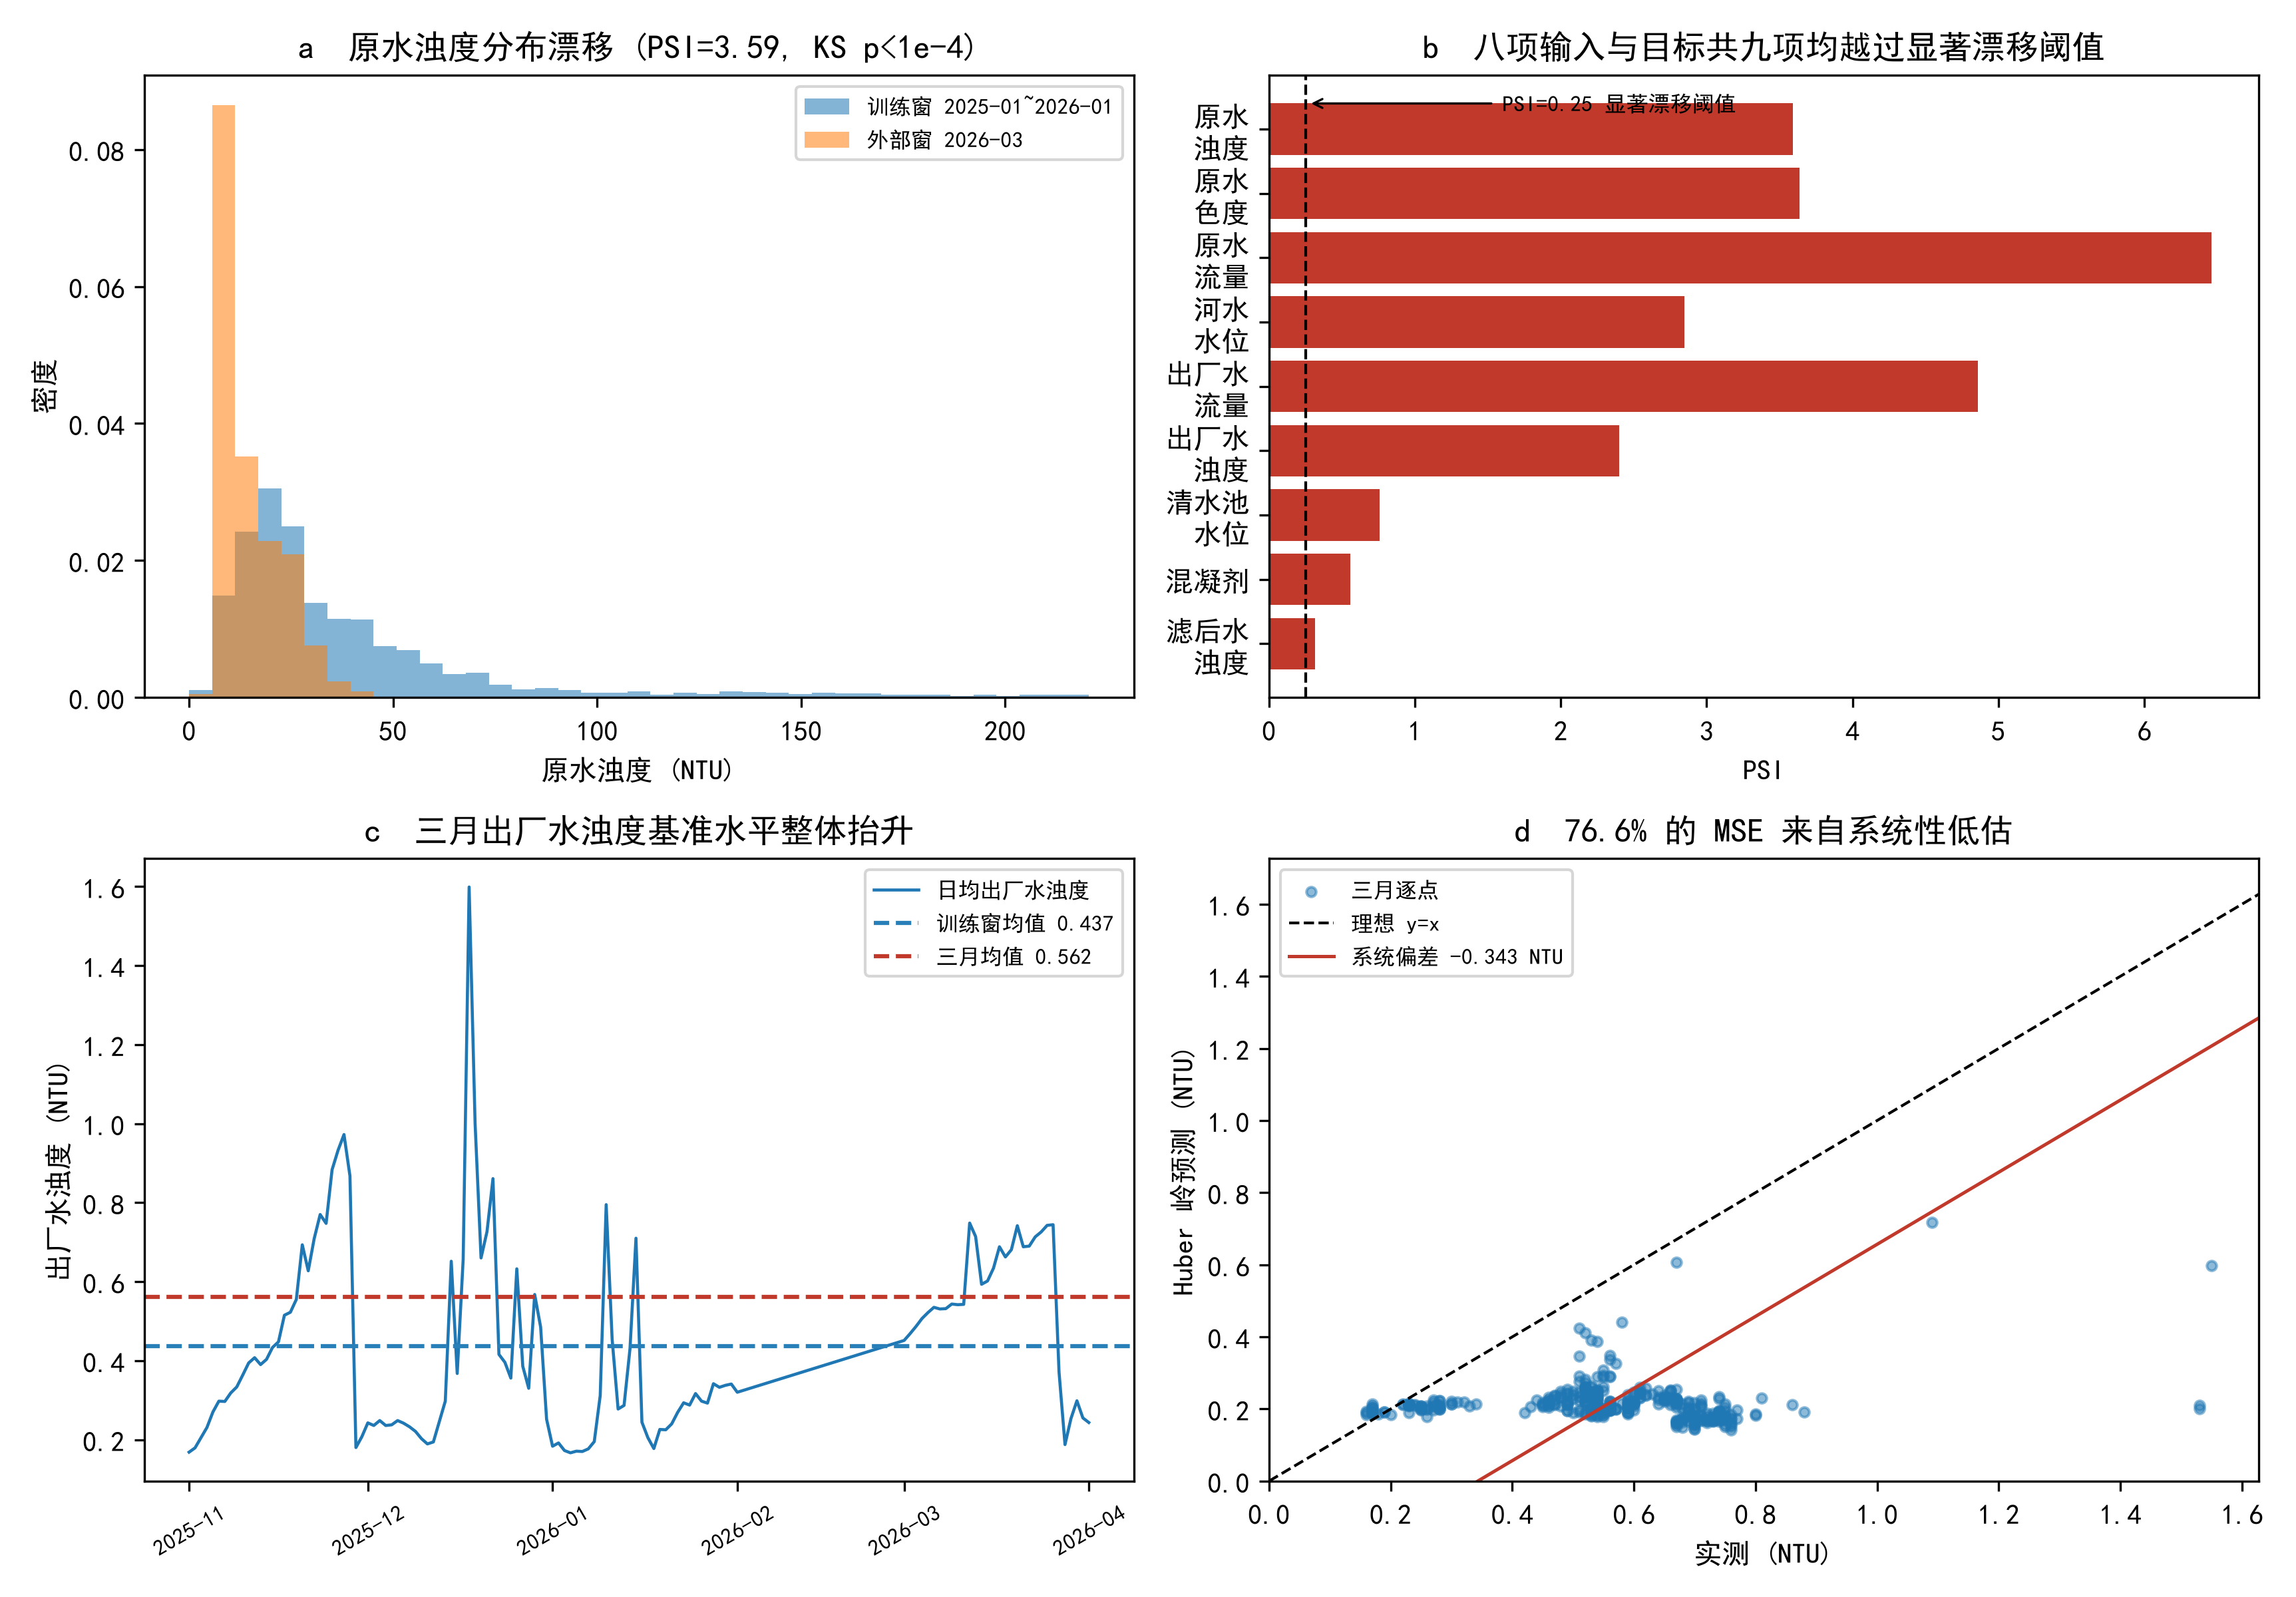
\includegraphics[width=0.95\textwidth]{diag_distribution_shift.png}
\caption{训练窗与 2026 年 3 月外部窗的分布漂移及问题一误差结构}
\label{fig:diag-shift}
\end{figure}

\begin{table}[htbp]
\centering
\caption{问题一 2026 年 3 月外部检验}
\label{tab:q1eval}
\begin{tabular}{lrrr}
\toprule
模型 & RMSE/NTU & MAE/NTU & $\Rtwo$\\
\midrule
Huber 岭 & 0.392112 & 0.345015 & $-3.447487$\\
RFF 岭 & 0.371614 & 0.318837 & $-2.994651$\\
同营运时次前一日 & 0.170873 & 0.065256 & 0.173359\\
\bottomrule
\end{tabular}
\end{table}

\section{问题二：滤后水动态响应和有效时滞}

\subsection{模型构建}

图~\ref{fig:q2-series} 显示原水与滤后水浊度相差一个至多个数量级，且滤后水偶尔出现尖峰。因此对两者使用对数尺度。设滤后水浊度为 $F_t$，四个外生输入为原水浊度、原水 pH、混凝剂投加量和原水流量，模型为
\begin{equation}
\log(1+F_t)=a_0+\sum_{k=1}^{p}\phi_k\log(1+F_{t-k})+
\sum_{m=1}^{4}h_m(X_{m,t-d_m})+\epsilon_t,
\label{eq:arx}
\end{equation}
其中 $h_m$ 包含一次项和平方项，并加入原水浊度与混凝剂、pH 与混凝剂的交互项，这就是所谓的 ARX 模型（AutoRegressive with eXogenous inputs)。$d_m$ 独立取 0、2、4、6 h，先对 $4^4=256$ 个组合和 5 个岭值做滚动搜索，再在 $p\in\{3,6,9,12\}$ 中选择自回归阶数。

该结构把两类动态分开：$\phi_k$ 描述滤后水自身的惯性和未显式观测的慢变化，$d_m$ 与 $h_m$ 描述外生输入在候选延迟后的条件贡献。同时，平方项允许输入在高、低区间具有不同斜率，两个交互项分别表示原水颗粒负荷与投药、酸碱状态与投药可能存在的协同变化。岭惩罚同时作用于自回归和外生系数，截距仍不惩罚。

即，对给定的 $\boldsymbol d=(d_1,\ldots,d_4)$、$p$ 和 $\lambda$，目标函数为
\begin{equation}
\min_{\boldsymbol\theta}\sum_{t\in\mathcal T}
\left[\log(1+F_t)-\boldsymbol z_t(\boldsymbol d,p)^{\mathsf T}\boldsymbol\theta\right]^2
+\lambda\|\boldsymbol\theta_{-0}\|_2^2.
\label{eq:arx-objective}
\end{equation}
候选时滞搜索先固定基础自回归结构，对 256 个组合分别考察 5 个岭值，共形成 1280 条验证记录；随后在选定时滞上比较 3、6、9、12 阶。这样的顺序既控制了计算规模，也使输入延迟与输出记忆长度的含义相对清楚。若一次性在所有阶数、交互形式和时滞上无约束搜索，有限的四个验证月容易选择到偶然最低点。

\begin{figure}[htbp]
\centering

\includegraphics[width=0.88\textwidth]{raw_q2_input_output_series.png}
\caption{2026 年 1--3 月原水与滤后水浊度序列}
\label{fig:q2-series}
\end{figure}

\subsection{时滞结果与鲁棒性分析}

图~\ref{fig:q2-lag} 中我们把另外两个输入和岭值取最优后，展示原水浊度与混凝剂时滞组合的滚动误差，可以得出最优输入时滞为原水浊度 2 h、原水 pH 0 h、混凝剂 0 h、原水流量 6 h，岭为 0.01，自回归阶数为 6。

为削弱序列趋势和低频扰动对相关分析的干扰，我们接着对时滞展开了互相关分析。

对于互相关分析，我们首先对四个输入变量和滤后水浊度进行一阶差分。对于原水浊度，先采用 \(\log(1+x)\) 变换，再计算相邻两个时次之差；其余变量直接进行一阶差分。由于数据采样间隔为 2 h，我们在 \(0\sim12\) h 范
围内依次计算
\[
\rho_j(k)=\operatorname{Corr}(\Delta X_{j,t-k},\Delta Y_t),
\qquad k=0,1,\ldots,6,
\]
并将绝对相关系数 \(|\rho_j(k)|\) 最大的位置记为变量 \(j\) 的互相关峰值时滞。该时
滞表示：在所考察的范围内，输入变量的短期变化与滤后水浊度变化在这一时间间
隔下具有相对较强的线性对应关系。

表~\ref{tab:q2lag} 显示，四个输入变量的互相关峰值绝对量仅为
\(0.0139\sim0.0408\)，均接近于 0，说明差分后单变量线性滞后关系较弱。因此，表中
时滞只能作为实际模型的候选时间尺度，不能视为精确辨识的物理输运时间。

原水浊度的 ARX 最优时滞为 2 h，而互相关峰位于 0 h，二者相差一个采样步；这表明原水浊
度的变化可能在当前或下一采样时次对滤后水浊度提供预测信息，但数据不足以进一步
区分其精确作用时刻。

原水流量的 ARX 最优时滞为 6 h，而互相关峰位于 2 h，二者相差两个采样步。该差异说明，单独观察原水流量时，其短期变化与 2 h 后的滤后水浊度变化对应较强；但在同时控制原水浊度、pH、混凝剂和滤后水浊度历史值
后，6 h 滞后对整体预测更有利。因此，6 h 可以代表多变量模型选择的有效预测位置，但也并
不意味着水体从原水端到过滤端的真实停留时间恰为 6 h。

原水 pH 和混凝剂的 ARX 最优时滞均为 0 h，其中混凝剂的互相关峰也位于 0 h，原
水 pH 的互相关峰位于 2 h。零时滞并不意味着水质变化能够瞬时完成物理传输，我们分析的结果是可
能反映同一班次内的联动控制过程：操作人员根据原水水质及时调整混凝剂投加量，使
原水指标、控制动作和滤后水响应在 2 h 采样网格上被记录为同一时次或相邻时次。
因此，这些结果体现的是“水质变化—操作调节—滤后响应”共同形成的统计时滞，而不是
单一水力过程的因果时滞。

\begin{figure}[htbp]
\centering

\includegraphics[width=0.53\textwidth]{process_q2_lag_search.png}
\caption{原水浊度与混凝剂时滞组合的最小滚动验证 RMSE}
\label{fig:q2-lag}
\end{figure}

\begin{table}[htbp]
\centering
\caption{问题二时滞与交叉相关检查}
\label{tab:q2lag}
\begin{tabular}{lrrr}
\toprule
输入 & ARX 时滞/h & 互相关峰/h & 峰值相关系数\\
\midrule
原水浊度 & 2 & 0 & 0.02443\\
原水 pH & 0 & 2 & 0.01392\\
混凝剂 & 0 & 0 & 0.02919\\
原水流量 & 6 & 2 & 0.04076\\
\bottomrule
\end{tabular}
\end{table}

\subsection{外部检验和分析}

我们使用 3 月的数据集进行外部检验，进一步验证模型效果。图~\ref{fig:q2-validation} 表明模型能跟随大部分低值水平，却不能稳定捕捉 3 月中旬的孤立尖峰。

实验结果显示， RMSE 为 0.166450 NTU、MAE 为 0.029398 NTU、$\Rtwo=-0.373590$。
通过分析可以看出，RMSE 与 MAE 的明显差距说明误差具有非均匀性，RMSE 约为 MAE 的 5.66 倍，少数大误差对平方损失贡献很高。若模型在所有时点都同等偏离，二者不会出现如此大的比例。结合外部检验图可知，常态低浊度段的大多数绝对误差较小，而尖峰的幅度或发生时刻未被正确预测。负 $\Rtwo$ 并不否定模型对常态水平的跟随能力，但表示在三月总体平方误差口径下，其增量解释不足。

同时，我们对自回归阶数敏感性也进行了分析。固定最优时滞和 $\lambda=0.01$ 时，3、6、9、12 阶的平均滚动 RMSE 分别为 0.530303、0.529050、0.529913 和 0.529717 NTU。6 阶相对 3 阶仅改善 0.001254 NTU，相对 9 阶也只低 0.000863 NTU；阶数增加并未带来单调收益。最终的 6 阶，即12 h 输出历史，是滚动 RMSE 标准下的最小值，但我们不能因此确定滤池过程恰好只需要 12 h，因为这一切仅仅只是当前数据反映的一种趋势。

从营运角度看，时滞结果可以用于安排观测窗口，而不能直接用于自动投药。例如原水流量的有效延迟为 6 h，提示评估某次流量变化时不宜只检查当前滤后水；原水浊度的 2 h 延迟则提示较快响应。但由于交叉相关很低、外部 $\Rtwo$ 为负，任何基于这些延迟的控制策略都应先在更长的时间段进行验证。特别是混凝剂与滤后浊度之间存在反向调节闭环，不能据简单的系数分析直接计算“增加多少药剂必然降低多少浊度”。

\begin{figure}[htbp]
\centering

\includegraphics[width=0.88\textwidth]{result_q2_external_validation.png}
\caption{ARX-Ridge 对滤后水浊度的 2026 年 3 月外部检验}
\label{fig:q2-validation}
\end{figure}

\section{问题三：清水池传播与出厂水浊度预测}

\subsection{质量守恒的停留时间分布}

首先，我们对数据进行初步分析，图~\ref{fig:q3-propagation} 显示清水池前后的短期波动并非简单平移，清水池具有混合和调蓄作用。因此，时刻 $t$ 的出厂水状态不仅受到
当前滤后水浊度的影响，还与此前一段时间进入清水池的滤后水有关。
为描述这种具有记忆性的传播过程，我们采用离散指数停留时间分布
构造物理传播模型。指数 RTD 是单个理想连续搅拌槽的基本情形，并具有滤除上游高频波动的作用\cite{toson2019}。
\begin{figure}[htbp]
\centering

\includegraphics[width=0.88\textwidth]{raw_q3_filtered_treated_series.png}
\caption{2026 年 1 月清水池前后浊度传播}
\label{fig:q3-propagation}
\end{figure}

设滤后水浊度为 $F_t$，采样间隔为 $\Delta t=2~\mathrm{h}$，
$\tau$ 为有效混合时间尺度。定义相邻滞后权重的衰减比为
\begin{equation}
q(\tau)=\exp\left(-\frac{\Delta t}{\tau}\right),
\qquad 0<q(\tau)<1.
\label{eq:rtd-decay}
\end{equation}
$\tau$ 越小，权重衰减越快，模型主要依赖近期滤后水；
$\tau$ 越大，历史信息保留时间越长，传播结果也越平滑。

无限指数核前 $J$ 项的累计质量为 $1-q^J$。为保留至少
$95\%$ 的核质量，取
\begin{equation}
J(\tau)
=
\min\left\{
m\in\mathbb{N}^{+}:1-q(\tau)^m\geq0.95
\right\}
=
\left\lceil
\frac{\log(0.05)}{\log q(\tau)}
\right\rceil.
\label{eq:rtd-length}
\end{equation}

截断后对各项权重重新归一化，得到
\begin{equation}
k_j(\tau)
=
\frac{q(\tau)^j}
{\displaystyle\sum_{r=0}^{J(\tau)-1}q(\tau)^r},
\qquad
j=0,1,\ldots,J(\tau)-1.
\label{eq:rtd-weight}
\end{equation}

归一化步骤消除了有限记忆窗口造成的系统性质量损失。综上，由此可得清水池传播的物理模型
\begin{equation}
P_t
=
\sum_{j=0}^{J(\tau)-1}
k_j(\tau)F_{t-j},
\qquad
\sum_{j=0}^{J(\tau)-1}k_j(\tau)=1.
\label{eq:rtd}
\end{equation}

式~\eqref{eq:rtd}表明，$P_t$ 是当前及历史滤后水浊度的加权平均。
其中，$k_0$ 对应当前滤后水，$k_1$ 对应 $2~\mathrm{h}$ 前的滤后水，
其余权重依次对应更早的观测值。由于各权重非负且总和严格等于 1，
若一段时间内 $F_t$ 恒为常数 $c$，则必有 $P_t=c$，因此传播过程
不会无故放大或缩小恒定的浊度水平。

接着，我们在候选集合
\[
\mathcal{T}=\{2,4,6,\ldots,24\}~\mathrm{h}
\]
中选择有效混合时间尺度。对于每个候选值 $\tau$，分别构造
对应的指数核和物理传播模型，并计算四折滚动验证的平均 RMSE，
最终取
\begin{equation}
\tau_0
=
\arg\min_{\tau\in\mathcal{T}}
\frac{1}{4}
\sum_{\ell=1}^{4}
\operatorname{RMSE}_{\ell}(\tau).
\label{eq:rtd-selection}
\end{equation}

计算结果表明，$\tau=8~\mathrm{h}$ 时平均验证 RMSE 最小，
为 $0.534302~\mathrm{NTU}$，故将其选为基准有效混合时间尺度。
此时 $q=\exp(-0.25)\approx0.7788$，$J=12$，截断前累计质量为
$1-q^{12}\approx0.9502$。

图~\ref{fig:q3-rtd} 左侧展示 $\tau=8~\mathrm{h}$ 时各滞后时点的
离散核权重，可以看出权重随滞后时间增加而逐步衰减；右侧比较
不同候选 $\tau$ 的四折平均验证 RMSE，并在 $\tau=8~\mathrm{h}$
处取得最小值。需要说明的是，$\tau$ 是由现有数据和验证准则确定的
有效混合时间尺度，并非通过池体容积与流量直接测得的真实水力停留时间。
\begin{figure}[htbp]
\centering

\includegraphics[width=0.88\textwidth]{process_q3_rtd_selection.png}
\caption{指数 RTD 核及有效混合时间尺度选择}
\label{fig:q3-rtd}
\end{figure}

\subsection{对数残差修正}

同时，我们考虑到纯 RTD 基线不能表达投药、流量等短期状态的偏离，故选择对目标的对数残差使用模型进行修正。

定义 $R_t=\log(1+Y_t)-\log(1+P_t)$，对每个偶数时距 $h\in\{2,4,6,8,10,12\}$ 分别建立模型
\begin{equation}
\log(1+\widehat Y_{t+h})=\log(1+P_{t+h})+f_h
\left(R_t,\ldots,R_{t-10\mathrm{h}},U_t\right),
\label{eq:hybrid}
\end{equation}
其中 $U_t$ 包含原水浊度、滤后水浊度、混凝剂、原水和出厂流量以及时次正余弦项，$f_h$ 为滚动选择岭值的 Huber 回归。

时次的正余弦编码为
\begin{equation}
c_t^{\ast}=\cos\left(2\pi s_t/12\right),\qquad
s_t^{\ast}=\sin\left(2\pi s_t/12\right),
\end{equation}
其中 $s_t=0,\ldots,11$ 表示营运日内时次。循环编码使 05:00 与下一营运日 07:00 在特征空间连续，不会因整数编码首尾相距 11 而产生伪时间距离。

我们对残差层选择使用对数尺度主要是由于浊度非负且偶有高值，直接使用原尺度的误差在高、低水平下方差差异明显。

另外，对于六个偶数时距，我们采用直接预测而非把 2 h 模型反复迭代到 12 h。直接模型允许不同 $h$ 使用不同系数和岭强度，避免单步偏差造成的机械累积。我们最终选择的岭参数按 2、4、6、8、10、12 h 依次为 1、1、10、10、1、1。另一方面，二月完整轨迹生成仍需随时间推进，因此我们在每个新时间点把模拟出的 $Y$ 写回最近残差状态。这形成“直接时距校正 + 逐时轨迹递推”的组合：前者服务于不同的预测时距，后者则保证整月风险评价拥有时间上连续且内部相关的样本路径。

\subsection{联合轨迹生成}

我们进一步考虑到，前面所述模型的确定性输出只能给出各时点的中心预测，不能反映未观测工况、
测量噪声和模型偏差造成的预测不确定性，这将容易造成水质序列中连续偏高或连续偏低的时间结构，并可能错误估计连续超标时长和日累计超标负荷。因此，我们选择利用历史回测误差构造
联合未来轨迹，而不是将相互独立的逐时预测区间直接拼接成未来轨迹曲线。具体而言，就是我们利用 1 月的历史回测误差帮助修正 2 月的预测结果。

具体而言，我们对于2026 年 1 月的每个回测起点 $t$，分别计算
$\mathcal H=\{2,4,6,8,10,12\}\,\mathrm{h}$ 六个预测时距的
对数尺度误差：
\begin{equation}
e_{t,h}
=
\log(1+Y_{t+h})-\widehat{\eta}_{t,h},
\qquad h\in\mathcal H,
\label{eq:horizon-error}
\end{equation}
其中，$Y_{t+h}$ 为实际出厂水浊度，$\widehat{\eta}_{t,h}$ 为模型
在对数尺度上的确定性预测。将同一预测起点的六个误差组成联合误差向量
\begin{equation}
\boldsymbol e_t=
\left(
e_{t,2},e_{t,4},e_{t,6},
e_{t,8},e_{t,10},e_{t,12}
\right).
\label{eq:joint-error}
\end{equation}
该向量保留了同一工况下不同预测时距误差之间的相关性。例如，当模型
在某个起点低估了 $2~\mathrm{h}$ 后的浊度时，其 $4~\mathrm{h}$ 和
$6~\mathrm{h}$ 预测也可能同时偏低，因而不能将六个误差分别抽样。

进一步我们考虑了相邻预测起点误差之间的时间依赖。由于采样间隔为
$\Delta t=2~\mathrm{h}$，我们取了连续 $L=12$ 个预测起点构成一个
移动误差块：
\begin{equation}
\mathcal B_s=
\left(
\boldsymbol e_s,
\boldsymbol e_{s+1},
\ldots,
\boldsymbol e_{s+L-1}
\right),
\qquad L=12.
\label{eq:error-block}
\end{equation}
每个误差块约覆盖 $12\times2=24~\mathrm{h}$，与一个营运日的时间
尺度相对应。重采样时有放回地随机抽取多个误差块并依次拼接，同时保持
每个块内部的时间顺序不变，这样就形成了一条长期的历史回测误差序列。

与逐时独立抽样相比，移动块重采样保留了两类相关结构：一是同一预测
起点下不同预测时距之间的联合误差关系；二是相邻时点连续偏高、连续偏低
或逐步恢复的时间变化特征。它重新组合的是历史滚动回测中真实出现过的
误差片段，而不是人为假设相互独立且服从正态分布的随机噪声。

最后，我们假设第 $b$ 次重采样得到的误差序列为
$\{\boldsymbol e_t^{(b)}\}$，则第 $b$ 条未来轨迹在时距 $h$ 处的
模拟值为
\begin{equation}
Y_{t+h}^{(b)}
=
\max\left\{
0,\,
\exp\left[
\widehat{\eta}_{t,h}+e_{t,h}^{(b)}
\right]-1
\right\},
\qquad
b=1,\ldots,B,
\label{eq:path}
\end{equation}
其中，$B=500$ 为重采样路径数。式~\eqref{eq:path}先在对数尺度上
将历史误差叠加到中心预测，再反变换至 NTU 尺度，并通过零下截断保证
浊度预测非负。

对于任一预测时点，将 500 条轨迹的模拟值从小到大排列，并分别取
$2.5\%$、$50\%$ 和 $97.5\%$ 分位数：
\begin{equation}
\widehat Y_t^{\,L}=Q_{0.025}
\left(\{Y_t^{(b)}\}_{b=1}^{B}\right),
\quad
\widehat Y_t=Q_{0.50}
\left(\{Y_t^{(b)}\}_{b=1}^{B}\right),
\quad
\widehat Y_t^{\,U}=Q_{0.975}
\left(\{Y_t^{(b)}\}_{b=1}^{B}\right).
\label{eq:path-quantiles}
\end{equation}
其中，$\widehat Y_t$ 为预测中位数，
$[\widehat Y_t^{\,L},\widehat Y_t^{\,U}]$ 为基于历史回测误差的
$95\%$ 预测区间。
\subsection{回测误差分析}

表~\ref{tab:q3acc} 与图~\ref{fig:q3-accuracy} 给出 3 月滚动起点回测。混合模型指前文所述的完整模型，纯物理基线指单纯使用指数停留时间模型 RTD 进行预测，持续性模型则指单纯认为水浊度 NTU 会保持当前值不变，作为最简单的基线进行比较。

混合模型在 2、4、6、8、10 h 均未超过持续性模型，只有 12 h 的 RMSE 0.139042 略小于持续性的 0.142469。纯物理基线 RMSE 约 0.52--0.54 NTU，说明 RTD 更适合作为物理结构基线而非独立精确预测器。分时距比较揭示了两种误差来源。2 h 时持续性 RMSE 为 0.092239 NTU，混合模型为 0.097030 NTU，差值仅 0.004791 NTU，表明出厂水短期惯性已很强，复杂特征没有提供稳定增益。到 8 h，二者差距扩大到 0.016773 NTU，混合修正仍未胜出。12 h 时混合模型比持续性低 0.003427 NTU，相对改善约 2.41\%，出现优势反转，这里可以看出短期惯性需要大约 10 h 进行消化，这与物理基线中给出的$\tau=8~\mathrm{h}$结果相似。

尽管绝对误差比较并不占优，混合模型在外部回测的 $\Rtwo$ 仍为 0.344--0.728，说明它能解释三月部分时序变化。这与 RMSE 基线结果并不矛盾：$\Rtwo$ 是相对检验集均值的比较，而持续性利用当前真实值，通常比均值强得多，所以后续我们可能需要更严格的持续性基线进行比较。

\begin{table}[htbp]
\centering
\caption{问题三分时距外部回测}
\label{tab:q3acc}
\begin{tabular}{rrrrr}
\toprule
时距/h & 物理 RMSE &混合 RMSE & 持续性 RMSE & 混合 $\Rtwo$ \\
\midrule
2 & 0.523008 &0.097030 & 0.092239 & 0.727982 \\
4 &0.530986& 0.136679 & 0.131063 & 0.460999 \\
6 & 0.534363&0.150911 & 0.137517 & 0.343940 \\
8 & 0.536191&0.142009 & 0.125236 & 0.420173 \\
10 & 0.536550&0.125370 & 0.120492 & 0.549029 \\
12 & 0.537052&0.139042 & 0.142469 & 0.446533\\
\bottomrule
\end{tabular}
\end{table}

\begin{figure}[htbp]
\centering

\includegraphics[width=0.53\textwidth]{result_q3_horizon_accuracy.png}
\caption{混合模型、持续性和纯物理基线的分时距 RMSE}
\label{fig:q3-accuracy}
\end{figure}

\subsection{实验预测结果和敏感性分析}
题目指定的 21 个时点均采用统一的 12 h 超前时间预测，即目标为 07:00 时，预测起点
是前一日 19:00；目标为 19:00 时，预测起点是当日 07:00。表~\ref{tab:q3designated}
给出混合模型基于 500 条联合轨迹得到的预测中位数及 95\% 预测区间。

\begin{table}[htbp]
\centering
\small
\caption{第三题指定日期 07:00--19:00 的 12 h 超前 NTU 预测}
\label{tab:q3designated}
\resizebox{\textwidth}{!}{%
\begin{tabular}{ccccccc}
\toprule
& \multicolumn{2}{c}{2 月 1 日} & \multicolumn{2}{c}{2 月 10 日} & \multicolumn{2}{c}{2 月 20 日}\\
\cmidrule(lr){2-3}\cmidrule(lr){4-5}\cmidrule(lr){6-7}
时刻 & 中位数 & 95\% 预测区间 & 中位数 & 95\% 预测区间 & 中位数 & 95\% 预测区间\\
\midrule
07:00 & 0.349445 & [0.047205, 0.885472] & 0.343118 & [0.088974, 1.457518] & 0.514015 & [0.029481, 1.436262]\\
09:00 & 0.341578 & [0, 1.111809] & 0.342581 & [0.088693, 1.200766] & 0.497372 & [0.002322, 1.414797]\\
11:00 & 0.347835 & [0, 1.018936] & 0.347700 & [0.085134, 1.183479] & 0.460659 & [0, 1.285575]\\
13:00 & 0.334371 & [0, 0.742681] & 0.353612 & [0.096335, 1.149050] & 0.435837 & [0.007598, 1.197847]\\
15:00 & 0.338348 & [0, 0.747664] & 0.377936 & [0.130712, 1.167902] & 0.434753 & [0.066085, 1.281363]\\
17:00 & 0.336115 & [0, 0.932885] & 0.396616 & [0.129112, 1.188549] & 0.427150 & [0.052483, 1.257316]\\
19:00 & 0.333276 & [0, 0.781374] & 0.400019 & [0.133130, 1.147793] & 0.423020 & [0.123903, 1.200217]\\
\bottomrule
\end{tabular}
}
\end{table}

2 月 1 日的中位数仅在 0.333276--0.349445 NTU 间小幅波动，日均为
0.340138 NTU，表现为低位平稳；2 月 10 日由早间约 0.343 NTU 逐步升至
19:00 的 0.400019 NTU，日均为 0.365940 NTU；2 月 20 日则由 07:00 的
0.514015 NTU 持续回落到 19:00 的 0.423020 NTU，但日均仍达 0.456115 NTU，
是三天中整体最高的一天。同时，我们发现三日的水力 RTD 基线日均分别为 0.109235、0.131700 和
0.108190 NTU，残差修正贡献日均分别为 0.230904、0.234240 和 0.347925 NTU，
说明仅靠 RTD 传播会系统性低估实际水平，数据驱动修正承担了主要的水平校正。

21 个预测中位数均低于 1 NTU，但有 16 个时点的 95\% 预测区间上界超过
1 NTU，其中 2 月 1 日为 2/7，2 月 10 日和 2 月 20 日均为 7/7。因此结果只能
说明中心轨迹处于低浊度区间，不能据此作确定性安全判断；较宽区间同时反映了
二月出厂水实测整段缺失、递推误差传播及跨月份残差不确定性。

敏感度分析只改变指定输入并保持其他历史和模型参数不变，回答的是局部条件敏感性而非干预效应。表~\ref{tab:q3sensitivity12h} 汇总三个起点的 12 h 结果。以 2 月 1 日起点为例，原水浊度增加 100\% 时，12 h 中心值由 0.322272 变为 0.329068 NTU，差约 0.006796 NTU；同日起点混凝剂减少 10\% 时，12 h 差约 $-0.000771$ NTU。变化相对预测区间很小。

我们发现，表~\ref{tab:q3sensitivity12h} 中显示混凝剂敏感性近乎为零，分析可得，其成因并不在模型形式，而在数据本身的信息量。训练窗内该字段共 3104 个有效值，却只出现 5 个不同取值；其中 0.05 出现 1617 次、0.06 出现 1467 次，两个相邻档位合计占 99.36\%，其余 0.04、0.07、0.08 三档合计仅 20 次。也就是说，投加量在记录中实际上只在两个相邻档位之间切换，既没有覆盖足够宽的剂量范围，也没有与浊度变化解耦的独立扰动。模型因此没有机会学到任何有意义的剂量--响应关系，表中近零的敏感性反映的是数据信息量不足，而不是“投药对出厂浊度没有影响”这一物理结论。这也与我们之前提到的立场相关，由于数据集分布可能存在偏移，我们不能据该敏感性制定或调整投药控制方案；若要识别真实剂量效应，需要在更宽剂量范围上进行受控试验，而非在现有观测上继续加大模型复杂度。

另外，上述扰动中我们只改变 07:00 起报点的一个当前输入，不能代表原水污染持续多个时次的
阶跃过程；同时，矾投加通常由原水水质触发调整，存在明显控制闭环。因此表中
变化量只能解释为给定其他条件时的局部模型响应，不能据此得出“增加或减少矾量
将使出厂水浊度改变多少”的因果结论。需要注意的是，为了方便起见，敏感性计算中我们采用未叠加自助残差的确定性中心，因此表~\ref{tab:q3sensitivity12h} 的基线与表~\ref{tab:q3designated}
中 500 条轨迹的预测中位数可能略有差异。

综上，这表明现有模型和观测数据不足以支持精细投药优化，合理用途是检验预测对输入扰动是否异常敏感。



\begin{table}[htbp]
\centering
\small
\caption{07:00 单点输入扰动下的 12 h 局部灵敏度（NTU）}
\label{tab:q3sensitivity12h}
\begin{tabular}{lrrrrr}
\toprule
日期 & 基线 & 原水浊度 $+25\%$ & 原水浊度 $+100\%$ & 明矾 $+10\%$ & 明矾 $-10\%$\\
\midrule
2 月 1 日  & 0.322272 & 0.002154 & 0.006796 & 0.000000 & $-0.000771$\\
2 月 10 日 & 0.289894 & 0.002002 & 0.006373 & 0.000000 & $-0.000752$\\
2 月 20 日 & 0.313788 & 0.002229 & 0.006979 & 0.000639 & 0.000000\\
\bottomrule
\end{tabular}
\end{table}
\section{问题四：营运日风险评估}

\subsection{幅度、时长与负荷指标}

设营运日 $d$ 的 12 个出厂水浊度为 $Y_{d,r}$，以 1 NTU 为基准定义超额
\begin{equation}
e_{d,r}=\max(Y_{d,r}-1,0),\quad
A_d=\max_re_{d,r},\quad
D_d=2\max\operatorname{run}(e_{d,r}>0),\quad
L_d=2\sum_re_{d,r}.
\label{eq:risk}
\end{equation}
其中 $A_d$ 为最大超标幅度，$D_d$ 为最长连续超标时长，$L_d$ 为 NTU$\cdot$h 意义下的超标负荷。若有效时点少于 9 个，则不直接评级；二月使用问题三的递推轨迹补充。

三个指标从不同角度描述同一天。$A_d$ 对单次高峰敏感，能够识别持续时间很短但幅度大的事件；$D_d$ 忽略幅度细节，强调超标是否连续；$L_d$ 同时累积幅度与持续时间，可区分两个最大值相同但整体负荷不同的营运日。2 h 系数来自采样间隔，因此 $D_d$ 只能取 0、2、4 h 等离散值。

设四个等级按 $0,1,2,3$ 编码，对第 $b$ 条路径得到 $G_d^{(b)}$，则二月的等级概率为
\begin{equation}
\widehat p_{d,g}=\frac{1}{500}\sum_{b=1}^{500}
\mathbf 1\{G_d^{(b)}=g\},\qquad g=0,1,2,3.
\label{eq:grade-probability}
\end{equation}
最终等级取概率最大的 $g$，区间则取 500 个有序等级的 2.5\% 和 97.5\% 分位位置。

分级规则为：$A_d=0$ 时 SAFE；$A_d\le0.5$ 且 $D_d\le4$ h 时 LOW；$A_d\le1.0$ 且 $D_d\le8$ h 时 MEDIUM；其他为 HIGH。该阈值是为了把幅度和持续时间进行联合编码。图~\ref{fig:q4-maximum} 给出每日最大值和 1 NTU 基准，图~\ref{fig:q4-matrix} 展示各日落在分级矩阵中的位置。

分级采用逐级包含的矩形边界。恰好等于 1 NTU 时超额为零并归 SAFE；最大超额不超过 0.5 NTU 且连续时长不超过 4 h 才可归 LOW，只要任一条件越界就进入更高等级判断。类似地，MEDIUM 要同时满足幅度不超过 1.0 NTU、时长不超过 8 h。逻辑中的“且”防止以很短时长掩盖过大峰值，也防止以很小幅度掩盖长时间连续超标。HIGH 是剩余集合，既包括大幅尖峰，也包括超过 8 h 的持续事件。

\begin{figure}[htbp]
\centering

\includegraphics[width=0.88\textwidth]{raw_q4_daily_maximum.png}
\caption{90 个营运日的最大出厂水浊度}
\label{fig:q4-maximum}
\end{figure}

\begin{figure}[htbp]
\centering

\includegraphics[width=0.53\textwidth]{process_q4_risk_matrix.png}
\caption{最大超标幅度与最长连续超标时长构成的风险矩阵}
\label{fig:q4-matrix}
\end{figure}

\subsection{等级结果与预测不确定性}

90 个营运日的众数等级分布见表~\ref{tab:q4}。3 月份的具体分类结果见表~\ref{tab:march-grade-result}。等级按照预设规则进行评判，例如，3 月 12 日实测最大浊度 1.55 NTU、最大超额 0.55 NTU、最长连续超标 4 h，判为 MEDIUM；3 月 13 日最大浊度 1.09 NTU、连续超标 2 h，判为 LOW。其余 3 月日均为 SAFE。


\begin{table}[htbp]
\centering
\caption{2026 年 1--3 月营运日等级分布}
\label{tab:q4}
\begin{tabular}{lrr}
\toprule
等级 & 天数 & 占比/\%\\
\midrule
SAFE & 86 & 95.56\\
LOW & 2 & 2.22\\
MEDIUM & 1 & 1.11\\
HIGH & 1 & 1.11\\
\bottomrule
\end{tabular}
\end{table}

\begin{table}[htbp]
  \centering
  \caption{2026年3月营运日风险分类结果}
  \label{tab:march-grade-result}
  \begin{tabular}{clrr}
  \toprule
  风险等级 & 对应日期 & 天数 & 占比/\% \\
  \midrule
  SAFE
  & 3月1日--11日、3月14日--31日
  & 29 & 93.55 \\
  LOW
  & 3月13日
  & 1 & 3.23 \\
  MEDIUM
  & 3月12日
  & 1 & 3.23 \\
  HIGH
  & 无
  & 0 & 0.00 \\
  \bottomrule
  \end{tabular}
  \end{table}

对每条二月轨迹独立评级，再由 500 个等级得到概率、众数和 2.5\%--97.5\% 等级范围。图~\ref{fig:q4-grades} 中竖线表示该范围。二月的中心轨迹均为 SAFE，但 28 天的等级上界没有一天停留在 SAFE：其中 6 天上界为 MEDIUM，22 天为 HIGH。这一结果与问题一的宽区间一致，说明“中心值低于 1 NTU”不能推出缺失月确定安全。

但，需要注意的是，等级区间较宽并不意味着二月实际发生了 22 个 HIGH 日，而是表示在历史误差块支持的联合轨迹中，这些日的高分位等级可以达到 HIGH。相反，众数为 SAFE 也不表示 HIGH 概率为零。中心值回答最典型轨迹的位置，等级上界回答尾部风险可能到达的类别。若营运决策对漏报高风险的代价远大于误报，则可关注 $P(G_d\ge \mathrm{MEDIUM})$；若用于常态资源安排，则还应结合众数、负荷中位数和最新在线观测。

另外，问题一与问题三对二月不确定性的用途不同。问题一给出三个指定营运日、12 个时次的条件预测，适合检查特定日内变化；问题三生成整月连续路径，适合计算连续超标和等级。两者模型结构、残差来源和目标不同，不能把问题一的逐点上下界直接替换问题三路径，但二者共同得到“中心偏低但上界宽”的结论。

\begin{figure}[htbp]
\centering

\includegraphics[width=0.88\textwidth]{result_q4_daily_grades.png}
\caption{90 个营运日的众数等级与 95\% 等级范围}
\label{fig:q4-grades}
\end{figure}

\section{模型评价}
\subsection{问题一：Huber 加权岭回归模型}

  优点：Huber 损失能够降低异常浊度值对参数估计的影响，岭惩罚可缓解水质变量及其滞
  后项之间的多重共线性。结合时间块置换重要度和滚动折方向一致性，可以筛选具有稳定
  预测贡献的变量，解释性较强。

  缺点：2026 年 2 月出厂水浊度完全缺失，无法直接校准该月模型。模型在 3 月外部检验中弱于前一营运日基线。但这并不是笼统的“泛化失败”，而是“水平定标失效、相对形态可用”，反映了跨月预测本身的难度和系统缺陷。此外，模型得到的是运行策略下的条件关联，不能因此将原水色度、矾投加量等变量的效应解释为因果作用。

 \subsection{ 问题二：带时滞搜索的 ARX-Ridge 模型}

  优点：模型同时考虑滤后水浊度的自回归惯性和原水浊度、pH、矾投加量、原水流量等外
  生变量的滞后影响，能够描述水处理过程的动态响应。通过滚动验证搜索时滞、自回归阶
  数和正则化参数，可避免仅凭相关系数人为指定延迟。

  缺点：与第一问类似，搜索得到的时滞是统计意义上的有效延迟，不等同于真实水力停
  留时间，因此也不能据此直接制定投药控制方案。

  \subsection{ 问题三：RTD 物理传播与 Huber 残差修正混合模型}

  优点：RTD 层满足非负性和质量守恒，能够解释滤后水经过清水池后的滞后和平滑过程；
  数据驱动层则修正理想水力模型无法描述的运行偏差。模型进一步生成500条联合预测轨
  迹，可同时给出预测中位数、95\%预测区间，并为问题四提供具有时间相关性的风险路
  径。

  缺点：单指数 RTD 难以描述旁路、分层、多池串联等复杂流态。混合模型仅在12 h时距
  略优于持续性基线，在2--10 h时距没有稳定优势。原水突变和明矾量调整也只检验了单点局部敏感性，不能代表持续污染过程造成的结果。

  \subsection{ 问题四：幅度—时长—负荷联合风险分级模型}

  优点：模型同时考虑最大超标幅度、最长连续超标时长和超标负荷，避免仅用日最大值评
  价水质风险。分级规则清晰、计算简单、便于现场解释，并利用问题三的500条轨迹给出
  等级概率、众数和区间，比单一确定性等级更加审慎。

  缺点：LOW、MEDIUM 和 HIGH 的边界属于针对本数据集的设计，不一定符合真实情况需求；临界日期可能因
  小幅预测误差发生等级跳变。二月等级高度依赖问题三的预测路径，因此会继承其参数误
  差、残差误差和模型结构误差。模型也未显式考虑降雨、反冲洗、设备切换等事件，不宜
  直接推广到更大规模水厂或直接作为自动控制规则。
\bibliographystyle{plain}
\bibliography{references}
\end{document}
